\section{Conclusion}
\label{sec:conclusions}
Summarization of the thesis and its contributions to the field.


\subsection{Disclaimers}
\label{sec:disclaimers}

\subsubsection{Plagiarism}
Substantial parts of some of the sections in the literature have been copy-pasted from a pre-thesis project of the same author as this thesis on the same subject from the preceding semester. The text has been partially rewritten and improved, but still share a high degree of similarity to the original content. This includes much of the text in sections \ref{sec:individual_privacy}, \ref{sec:object_detection}, \ref{sec:thirdparty_products}

\subsubsection{The Use of AI Tools}
Some of the code and text in this thesis has been enhanced by the use of AI tools. For the main portions of the writing process, Github Co-Pilot was considered mostly distracting and therefore disabled. In figure \ref{fig:co-pilot_distracting} we see an example of one of these distracting suggestions, where it may seem AI thinks very strongly we need more reasearch on who are not wearing masks and are not vaccinated... The somewhat humurous suggestion serves only as a distraction. 

\begin{figure}[H]
	\centering
	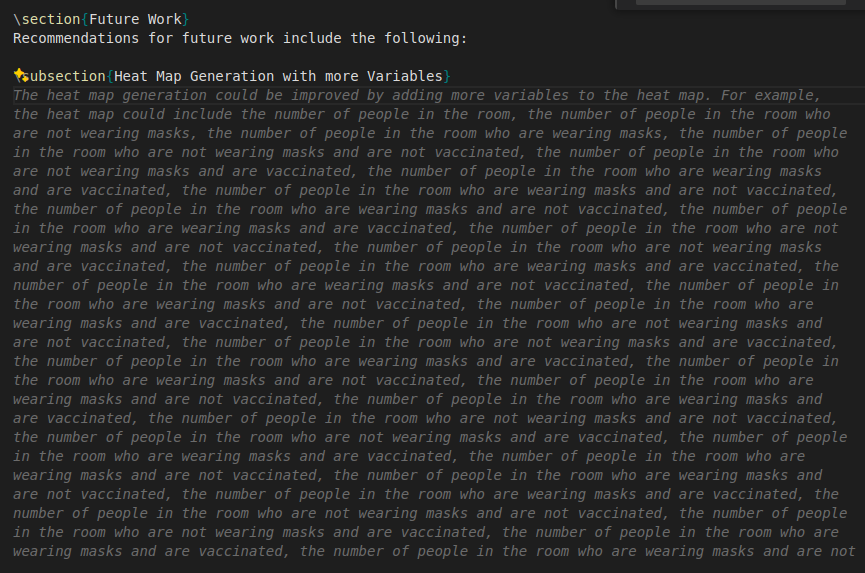
\includegraphics[width=\textwidth]{Images/Fun/co_pilot_distracting.png}
	\caption{The Co-Pilot is mostly annoying for Latex.}
	\label{fig:co-pilot_distracting}
\end{figure}

However, some boiler-plate Latex-code and some of the sections have been fed to an AI to verify it's quality and to get suggestions on how to enhance readability and flow. The tools used have been Chat-GPT4 by OpenAI and Github Co-Pilot.  

\subsubsection{Privacy of Similar Projects}
The author of this thesis is not an expert in privacy. The methods outlined in this thesis are meant to ensure privacy of individuals, but the author cannot guarantee that the methods are foolproof. The author has tried to follow best practices and guidelines from the field and has tried to be transparent about the methods used and the limitations of the methods, but the reader should be aware that following the methods outlined in this thesis may not necessarily be enough to ensure privacy. An investigation into the privacy of similar projects is recommended before deploying a similar system in a real-world setting.